\documentclass[conference]{IEEEtran}
\IEEEoverridecommandlockouts
% The preceding line is only needed to identify funding in the first footnote. If that is unneeded, please comment it out.
\usepackage{cite}
\usepackage{amsmath,amssymb,amsfonts}
\usepackage{algorithmic}
\usepackage{graphicx}
\usepackage[brazilian]{babel}
\usepackage[utf8]{inputenc}
\usepackage[T1]{fontenc}
\usepackage{textcomp}
\usepackage{listings}
\usepackage{graphicx}
\usepackage{float}

\def\BibTeX{{\rm B\kern-.05em{\sc i\kern-.025em b}\kern-.08em
    T\kern-.1667em\lower.7ex\hbox{E}\kern-.125emX}}
\begin{document}

\title{Simulação Biológica de Agrupamento de Formigas Mortas}

\author{\IEEEauthorblockN{1\textsuperscript{st} Marlon Henry Schweigert}
\IEEEauthorblockA{\textit{Departamento de Computação} \\
\textit{Centro de Ciências Tecnológicas - UDESC}\\
Joinville, Brasil \\
marlon.henry@magrathealabs.com}
\and
\IEEEauthorblockN{2\textsuperscript{nd} Rafael Stubs Parpinelli}
\IEEEauthorblockA{\textit{Departamento de Computação} \\
\textit{Centro de Ciências Tecnológicas - UDESC}\\
Joinville, Brasil \\
rafael.parpinelli@udesc.br}
}

\maketitle

\begin{abstract}
Este meta-artigo descreve o funcionamento computacional da simulação de formigas utilizando inteligência artificial dentro de um ambiente homogêneo visando simular o agrupamento de dados em lugares densos, realizando uma análise entre a variação dos parâmetros utilizados para o processamento da inteligência artificial.
\end{abstract}

\begin{IEEEkeywords}
formigas, inteligência artificial, modelagem matemática, programação concorrente
\end{IEEEkeywords}


\section{Introdução}

A busca por simular efeitos naturais que otimizem problemas em sistemas computacionais tem grandes vantagens comparados a algoritmos deterministas e objetivos, vistos que podemos dar sentido a resultados obtidos da natureza a qual algoritmos puramente matemáticos custam fazer qualquer sentido. Essa propriedade principal é aplicada ao algoritmo de aglomeração de formigas mortas por um grupo de formigas vivas.

O efeito de agrupamento de um ambiente poluído por formigas mortas é relatado por Mohamed Jafar~\cite{b1}, a qual tem um sistema matemático pode descrever a movimentação de tais agentes~\cite{b2}.

\begin{figure}[h]
\centering
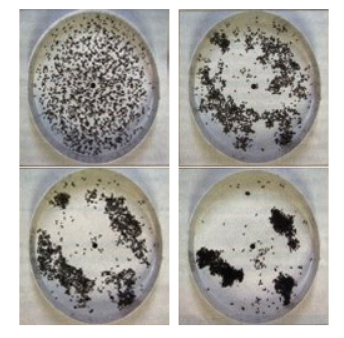
\includegraphics[width=2.5in]{clusters.png}
\caption{\textit{Clusters} de formigas mortas.}
\label{fig_sim}

Fonte: O. A. Mohamed Jafar, R. Sivakumar \cite{b1}
\end{figure}

Tal comportamento é conhecido como agrupamento, na qual esse efeito pode ser utilizado para otimizar problemas de agrupamento, limpeza ou desfragmentação de ambientes na qual os dados manipulados sejam homogêneos \cite{b1}.

Este artigo será dividido em duas grandes partes. A primeira grande parte contempla o agrupamento de formigas mortas como simulação biológica. As seções que contemplam a primeira grande parte são:

\begin{itemize}
    \item \textbf{Caracterização do problema}: Descreve a análise das características do problema e medidas de desempenho.
    \item \textbf{Modelagem matemática}: Descreve as ações e o modelo matemático a qual os agentes podem realizar.
    \item \textbf{Resultados obtidos}: Amostras estado de execução obtidos da modelagem descrita, assim como métricas de recursos utilizados.
    \item \textbf{Análise sobre resultados obtidos}: Análise sobre estados obtidos e modelagem descrita.
\end{itemize}

A segunda grande parte contempla a utilização desse fenômeno para agrupamento de dados utilizando critérios de diferença de dados. As suas seções são:

\begin{itemize}
    \item \textbf{Modelagem Matemática para dados}: Modelagem matemática para diferenciar dados favorecendo o agrupamento de dados.
    \item \textbf{Simulação e resultados obtidos para dados}: A execução e resultados obtidos utilizando tal abordagem.
\end{itemize}

\section{Caracterização do problema}

Para melhor entendimento do problema, faz necessário classificar o problema de agrupamento de formigas mortas. Para tal, precisamos definir quais suas características\cite{b1}.

A sua classificação segue o determinado padrão:

\begin{itemize}
    \item \textbf{Ambiente}: Matriz de formigas mortas e vivas.
    \item \textbf{Agente}: Formiga viva.
    \item \textbf{Sensores}: Analisar região em torno de sí própria por um raio $R$.
    \item \textbf{Atuadores}: Pegar e soltar formigas mortas.
    \item \textbf{Desempenho}: Quantidade de grupos formados.
\end{itemize}

Algumas características dessa simulação são:

\begin{itemize}
    \item Parcialmente observável;
    \item Estocástico;
    \item Sequencial;
    \item Dinâmico;
    \item Discreto;
    \item Multiagente;
\end{itemize}

\section{Modelagem matemática}

O ambiente onde ocorrerá a simulação é desenhado como uma matriz esférica, ou seja, conectada pelas pontas. A fim de descrever matematicamente o comportamento de agrupamento de formigas mortas em tal ambiente, precisamos tomar alguns conceitos de como o fenômeno ocorre\cite{b1}:

\begin{itemize}
    \item Sem comunicação entre agentes: As formigas não utilizam nenhum método de comunicação entre outras formigas vivas para realizar este comportamento.
    \item Esse comportamento sempre é executado visando melhorar o caminho do ambiente.
    \item As ações tomadas podem ser descritas como:
    \begin{itemize}
        \item Pegar formiga;
        \item Soltar formiga;
        \item Caminhar;
    \end{itemize}
    \item As únicas percepções que a formiga utiliza para tomada de decisão são:
    \begin{itemize}
        \item Densidade da região onde ela está, utilizando um raio de visão.
        \item Se em sua atual posição existe ou não uma formiga.
    \end{itemize}
\end{itemize}

Dada essas características, podemos modelar as ações da formiga como uma cadeia de Markov a qual suas ações futuras requerem do seu estado atual. Essa cadeia de Markov é exibida na figura \ref{fig:automata}.

\begin{figure}[ht]
\centering
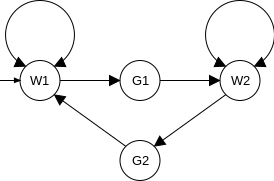
\includegraphics[width=2.5in]{how_walk_1.png}
\caption{Automato de estado de cada formiga.}
\label{fig:automata}
\end{figure}

Os estados descritos na figura \ref{fig:automata} são:

\begin{itemize}
    \item W1: Andando sem carregar uma formiga morta.
    \item G1: Pegar alguma formiga. Este estado tem uma probabilidade calculada dinamicamente conforme a posição atual da formiga.
    \item W2: Andando com uma formiga morta.
    \item G2: Soltar uma formiga morta. Este estado tem uma probabilidade calculada dinamicamente conforme o local da formiga.
\end{itemize}

Para este modelo funcionar, precisamos de um raio de visão ($R$), a qual significa quantas casas ao seu redor uma formiga pode observar. Esse parâmetro pode ser observado na figura \ref{fig:raio}.

\begin{figure}[h]
\centering
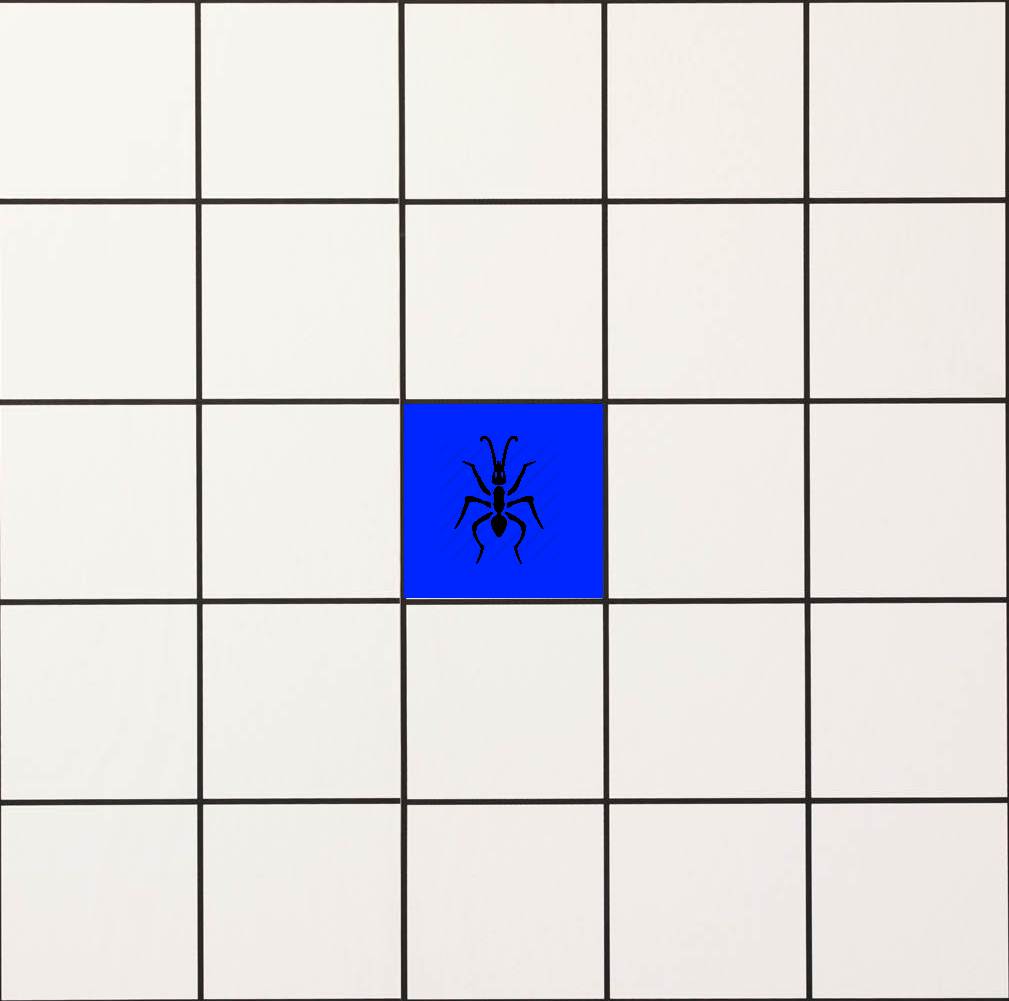
\includegraphics[width=2.5in]{formiga.png}
\caption{Formiga sobre a matriz, utilizando raio de visão 2.}
\label{fig:raio}
\end{figure}

O fator de decisão principal para pegar e soltar uma formiga morta está em torno da variável $D$ a qual é definida pela densidade local de cada formiga em torno do raio $R$ de cada formiga \cite{b2}.


$D = \sum_{i=-R}^{R}\sum_{j=-R}^{R}A(i,j)$, onde

$A(i,j) =
\begin{array}{ll}
    1, if(has\_ant\_at(i,j))\\
    0
\end{array}
$

A abordagem desta simulação utiliza uma memória para cada formiga onde é armazenado qual a maior densidade ($D_{max}$) a qual esta formiga encontrou em sua vivência com o ambiente de testes. Essa informação é útil para normalizar dentro de um valor real [0, 1] a variável de Densidade relativa ($D_{rel}$). A fórmula de normalização é dada por\cite{b2}:

$
    D_{rel} = \frac{D}{D_{max}}
$

Por fim, o modo de pensar da formiga é dado por tal algoritmo:

\lstinputlisting[language=Python]{ants.py}

Tal simulação foi criada em Golang para ter alto desempenho, facilidade de escritas de imagens e programação paralela facilitada.

Para funcionamento geral, executamos algumas threads onde cada thread manipula um conjunto de formigas. Cada formiga executará o algoritmo descrito acima por n vezes. Ao final, caso alguma formiga esteja carregando alguma formiga morta, elas executam paços até encontrarem um local bom para soltar e deixam de executar.

\section{Resultados Obtidos}

Utilizando $R=1$ foram obtidos as amostras (\ref{fig:r1}), a qual demonstram o agrupamento funcional mesmo pouca informação global para cada agente. Em comparativo a amostra obtida com $R=5$ (\ref{fig:r5}), as bordas são bem mais definidas no teste executado com $R=1$, porém em contra partida os grupos são mais definidos com $R=5$.

\begin{figure}[H] 
  \begin{minipage}[b]{0.5\linewidth}
    \label{fig:r1} 
    \centering
    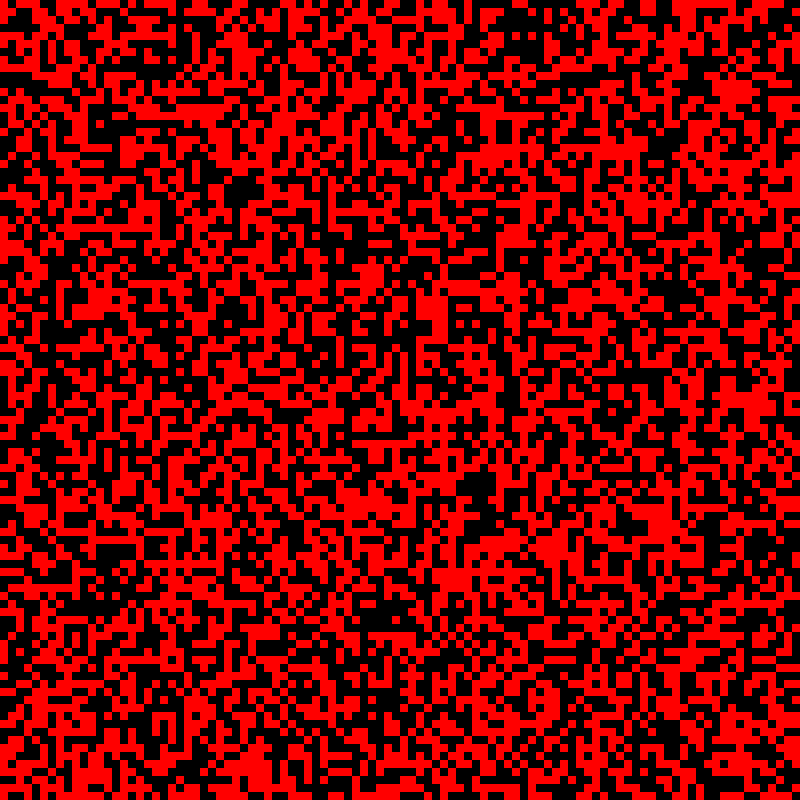
\includegraphics[width=.8\linewidth]{resultados/1-0.png} 
    \caption{Estado inicial com R=1} 
    \vspace{4ex}
  \end{minipage}%%
  \begin{minipage}[b]{0.5\linewidth}
    \centering
    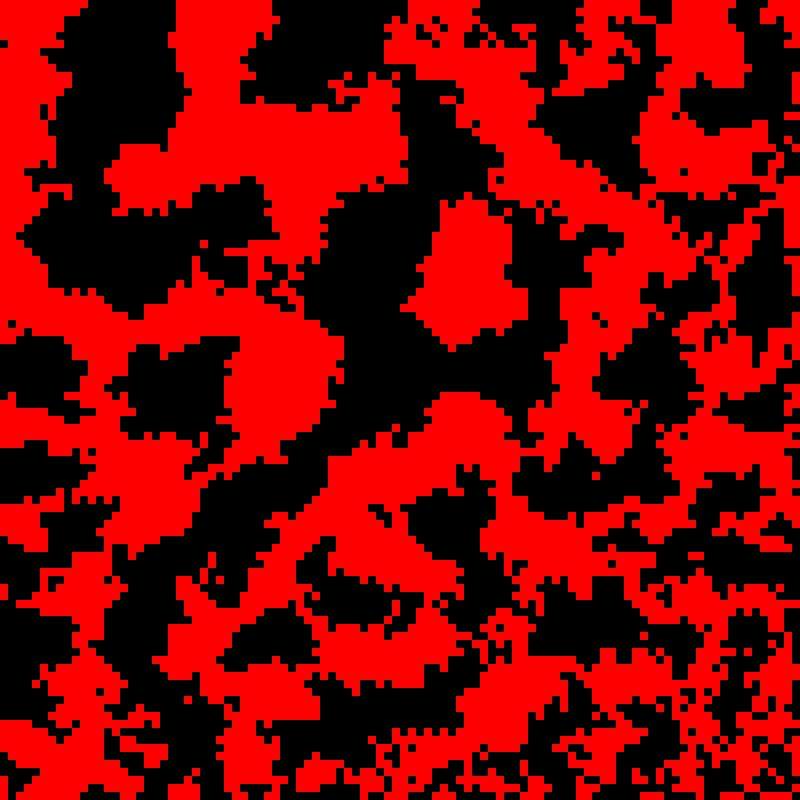
\includegraphics[width=.8\linewidth]{resultados/1-1.png} 
    \caption{100000 passos com R=1} 
    \vspace{4ex}
  \end{minipage} 
  \begin{minipage}[b]{0.5\linewidth}
    \centering
    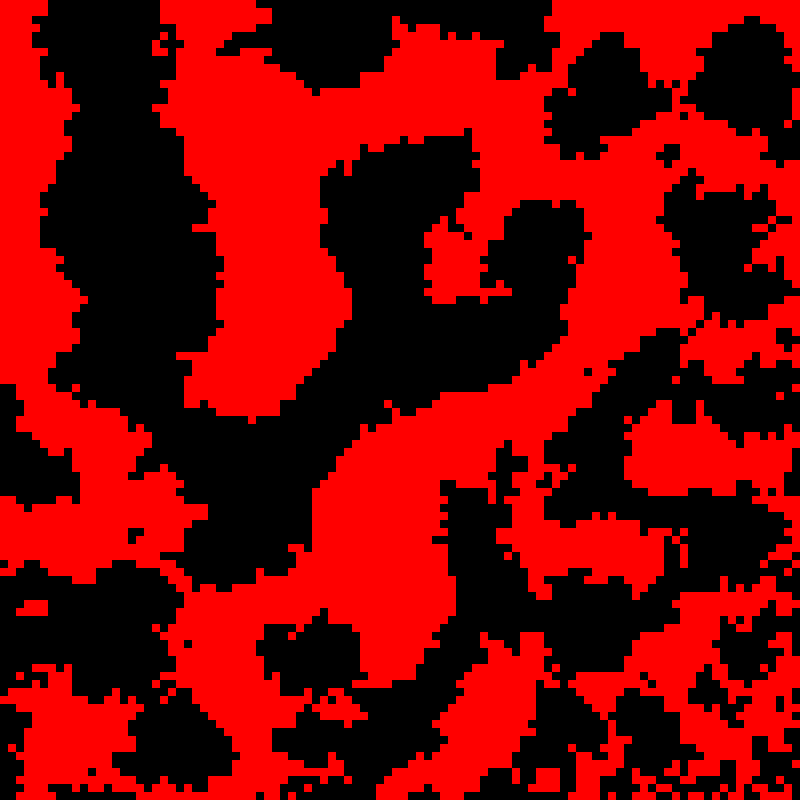
\includegraphics[width=.8\linewidth]{resultados/1-3.png} 
    \caption{300000 passos com R=1} 
    \vspace{4ex}
  \end{minipage}%% 
  \begin{minipage}[b]{0.5\linewidth}
    \centering
    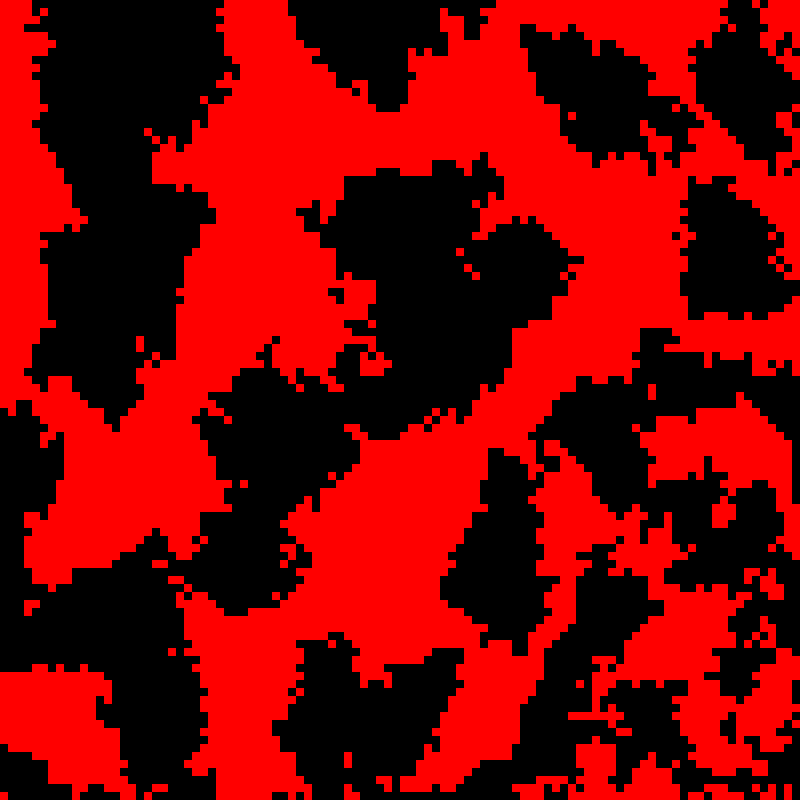
\includegraphics[width=.8\linewidth]{resultados/1-6.png} 
    \caption{500000 passos com R=1} 
    \vspace{4ex}
  \end{minipage} 
\end{figure}


A regra de aglomeração utilizando $R=1$ torna as bordas bem delimitadas e propicia a criação de grupos menores. O resultado final cria caminhos pequenos e tortuosos utilizando $R=1$ (figura \ref{fig:r1}.

\begin{figure}[H]
  \begin{minipage}[b]{0.5\linewidth}
    \label{fig:r5} 
    \centering
    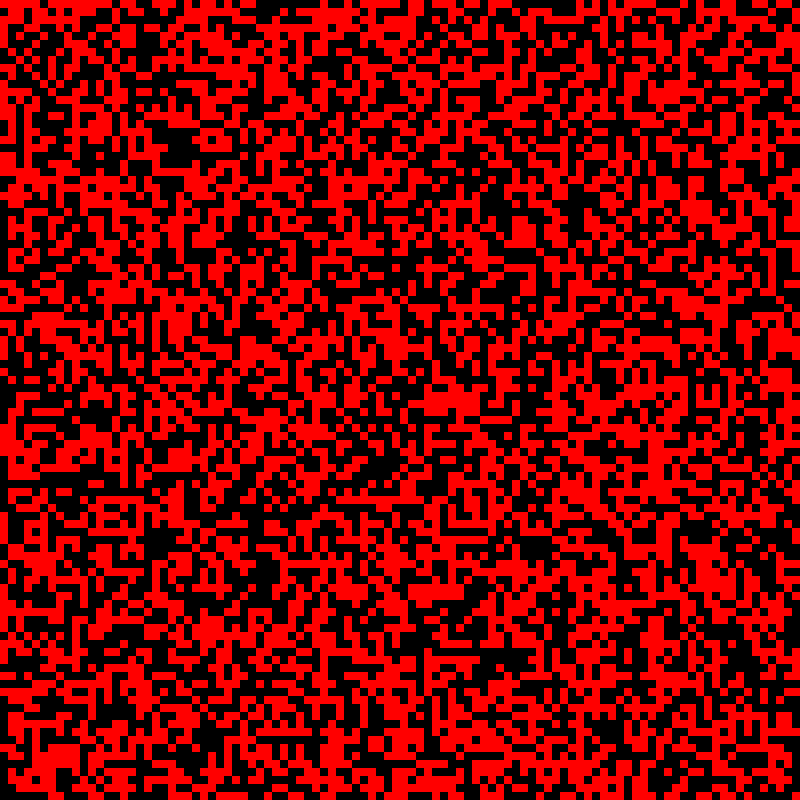
\includegraphics[width=.8\linewidth]{resultados/5-0.png} 
    \caption{Estado inicial com R=5} 
    \vspace{4ex}
  \end{minipage}%%
  \begin{minipage}[b]{0.5\linewidth}
    \centering
    
\includegraphics[width=.8\linewidth]{resultados/5-1.png} 
    \caption{100000 passos com R=5} 
    \vspace{4ex}
  \end{minipage} 
  \begin{minipage}[b]{0.5\linewidth}
    \centering
    
\includegraphics[width=.8\linewidth]{resultados/5-3.png} 
    \caption{300000 passos com R=5} 
    \vspace{4ex}
  \end{minipage}%% 
  \begin{minipage}[b]{0.5\linewidth}
    \centering
    
\includegraphics[width=.8\linewidth]{resultados/5-6.png} 
    \caption{500000 passos com R=5} 
    \vspace{4ex}
  \end{minipage} 
\end{figure}

A regra de aglomeração utilizando $R=5$ (figura \ref{fig:r5}) proporciona uma maior fragmentação dos grupos, mas ainda geram grupos bem definidos. Podemos perceber que a quantia de passos para as formigas formar grupos definidos é maior comparado ao teste de $R=1$ (figura \ref{fig:r1}).

\begin{figure}[H] 
  \begin{minipage}[b]{0.5\linewidth}
    \label{fig:r10}
    \centering
    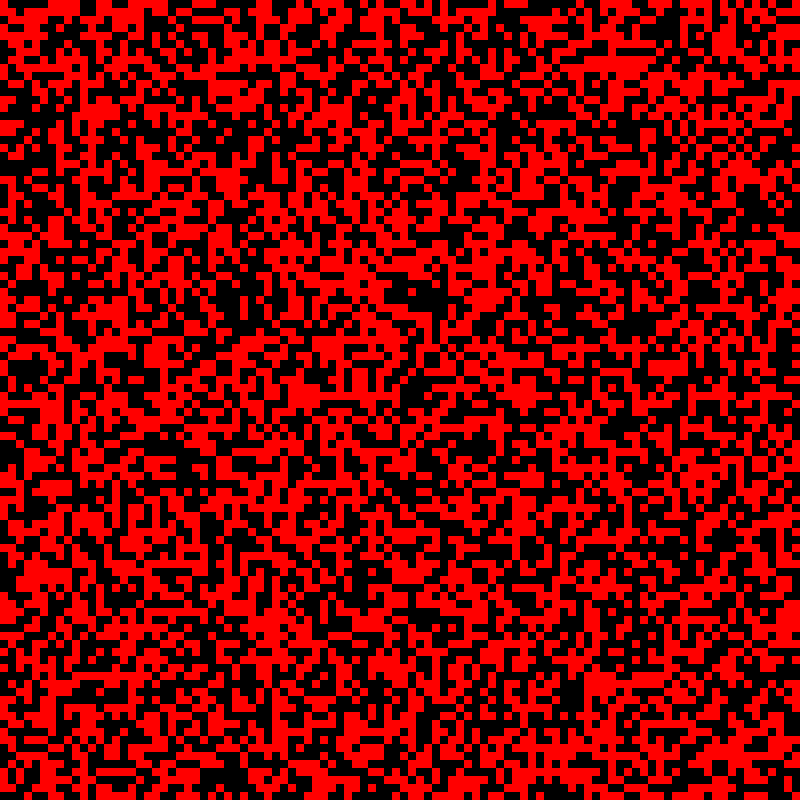
\includegraphics[width=.8\linewidth]{resultados/10-0.png} 
    \caption{Estado inicial com R=10} 
    \vspace{4ex}
  \end{minipage}%%
  \begin{minipage}[b]{0.5\linewidth}
    \centering
    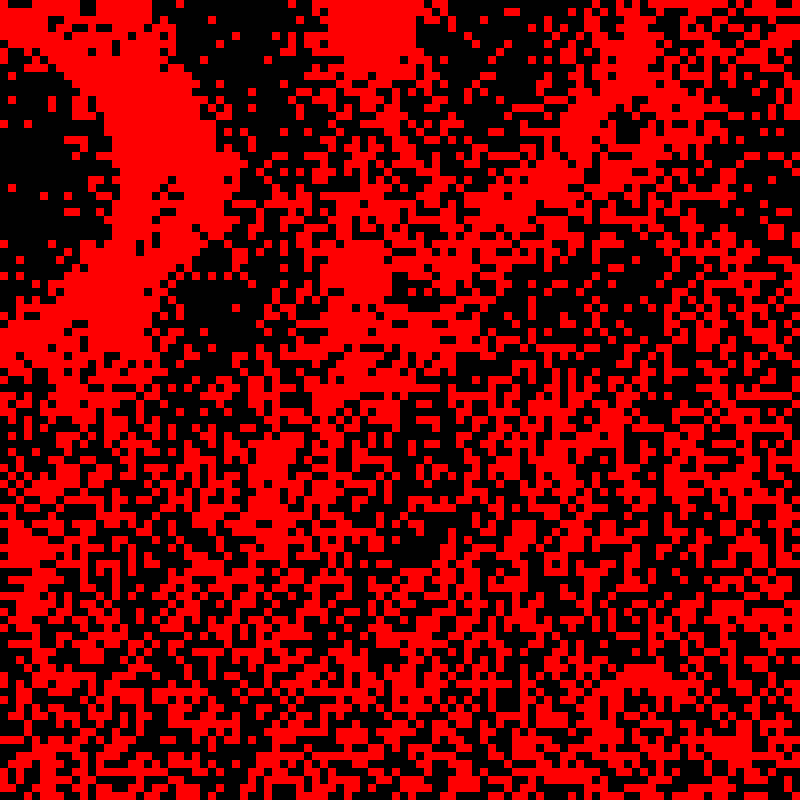
\includegraphics[width=.8\linewidth]{resultados/10-1.png} 
    \caption{100000 passos com R=10} 
    \vspace{4ex}
  \end{minipage} 
  \begin{minipage}[b]{0.5\linewidth}
    \centering
    
\includegraphics[width=.8\linewidth]{resultados/10-3.png} 
    \caption{300000 passos com R=10} 
    \vspace{4ex}
  \end{minipage}%% 
  \begin{minipage}[b]{0.5\linewidth}
    \centering
    
\includegraphics[width=.8\linewidth]{resultados/10-6.png} 
    \caption{500000 passos com R=10} 
    \vspace{4ex}
  \end{minipage} 
\end{figure}


Podemos ver um agravante na fragmentação das bordas dos grupos utilizando $R=10$ (\ref{fig:r10}). Além disso, podemos perceber que o agrupamento nos primeiros passos, entre 0 e 100000 passos é muito mais custoso a ocorrer comparado aos raios menores.

\begin{figure}[h]
  Comparativo entre estados finais com raios diferentes:
  

  \begin{minipage}[b]{0.5\linewidth}
    \label{fig:comp}
    \centering
    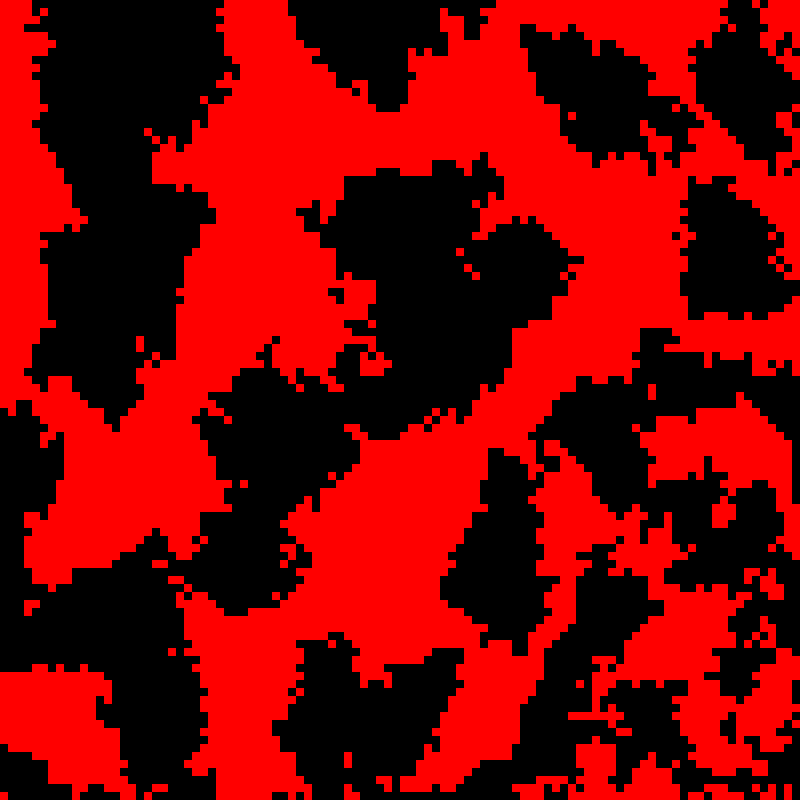
\includegraphics[width=.8\linewidth]{resultados/1-6.png} 
    \caption{500.000 passos com $R=1$} 
    \vspace{4ex}
  \end{minipage}%%
  \begin{minipage}[b]{0.5\linewidth}
    \centering
    
\includegraphics[width=.8\linewidth]{resultados/5-6.png} 
    \caption{500.000 passos com $R=5$} 
    \vspace{4ex}
  \end{minipage} 
  \begin{minipage}[b]{0.5\linewidth}
    \centering
    
\includegraphics[width=.8\linewidth]{resultados/10-6.png} 
    \caption{500.000 passos com $R=10$} 
    \vspace{4ex}
  \end{minipage}%% 
\end{figure}

\begin{table}[H]
\centering
\caption{Tabela de tempo de execução}
\label{table}
\begin{tabular}{|l|l|l|l|}
\hline
                            & R = 1  & R = 5   & R = 10    \\ \hline
Tempo médio de 10 execuções & 4.442s & 44.869s & 2m 4.401s \\ \hline
variação                    & 0.5\%  & 0.9\%   & 1.1\%     \\ \hline
\end{tabular}
\end{table}

Podemos assumir então, que quanto maior o raio, mais disperso será as bordas dos grupos. Isso é dado pela quebra de sistemas emergentes, visito que cada agente está levando em conta uma região muito grande ao invés de se preocupar com poucas informações. Essa comparação final é explicitada na figura~\ref{fig:comp}.

Além do resultado final não ser satisfatório, o tempo de execução não é bom quanto o esperado, comparando o resultado de raios menores com raios maiores. A complexidade $O(r²)$ para verificação da existência de formiga morta em uma determinada casa da matriz dificulta o tempo de execução quanto maior seja o raio das formigas vivas. 


\section{Análise dos resultados obtidos}

\begin{figure}[H] 
  \begin{minipage}[b]{0.5\linewidth}
    \label{fig:r_rand}
    \centering
    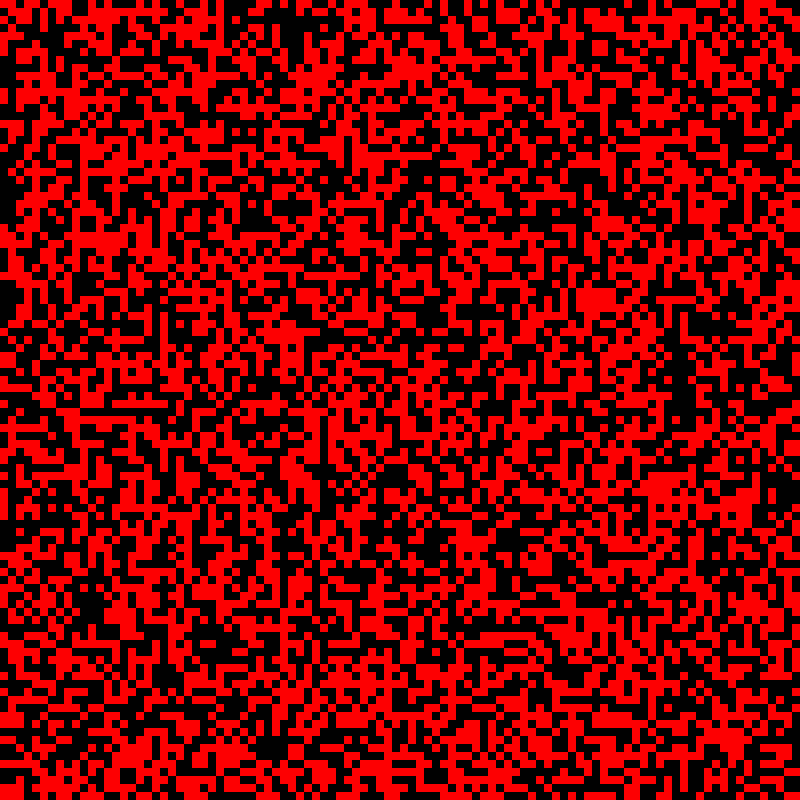
\includegraphics[width=.8\linewidth]{resultados/5-0-rand.png} 
    \caption{Estado inicial com $R=rand(5)+1$} 
    \vspace{4ex}
  \end{minipage}%%
  \begin{minipage}[b]{0.5\linewidth}
    \centering
    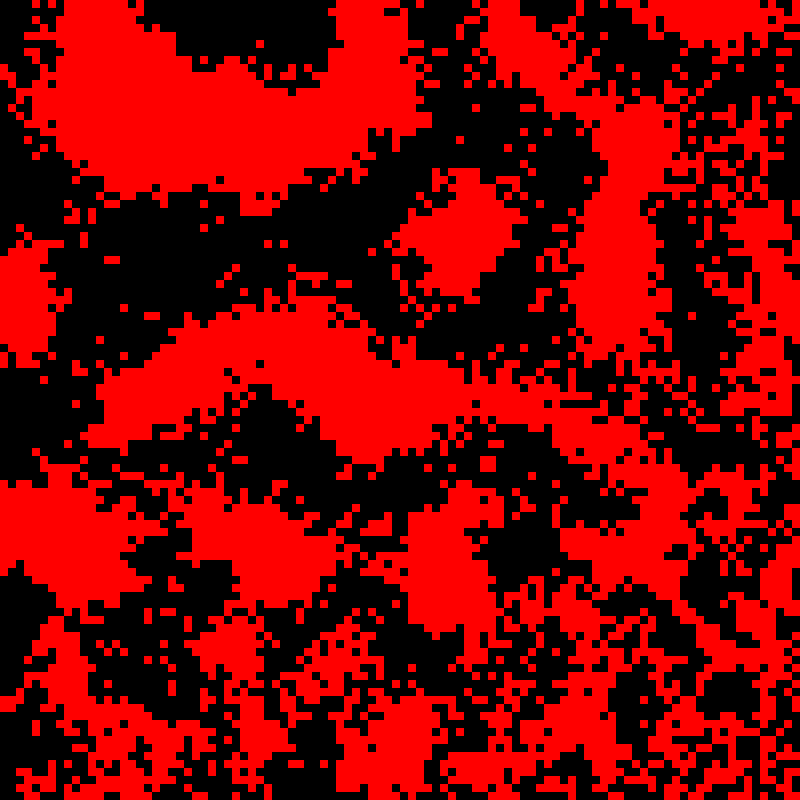
\includegraphics[width=.8\linewidth]{resultados/5-1-rand.png} 
    \caption{100000 passos com $R=rand(5)+1$} 
    \vspace{4ex}
  \end{minipage} 
  \begin{minipage}[b]{0.5\linewidth}
    \centering
    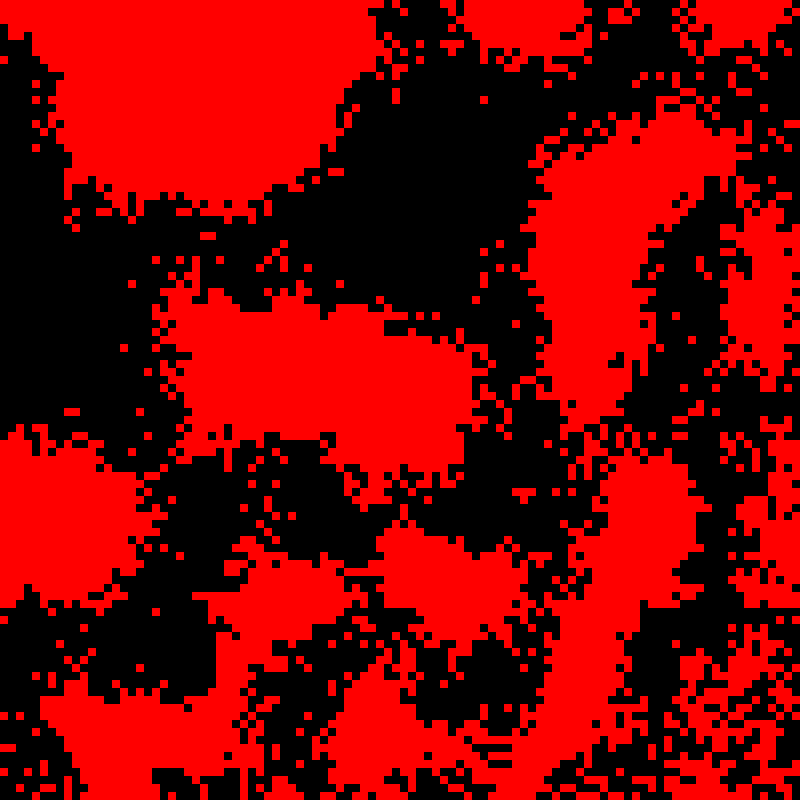
\includegraphics[width=.8\linewidth]{resultados/5-3-rand.png} 
    \caption{300000 passos com $R=rand(5)+1$} 
    \vspace{4ex}
  \end{minipage}%% 
  \begin{minipage}[b]{0.5\linewidth}
    \centering
    
\includegraphics[width=.8\linewidth]{resultados/5-6-rand.png} 
    \caption{500000 passos com $R=rand(5)+1$} 
    \vspace{4ex}
  \end{minipage} 
\end{figure}

Podemos concluir que, em sistemas emergentes, passar mais informação a ponto de quebrar a ideia de sistemas emergentes acaba dificultando a convergência do sistema.

Percebe-se que a variação $R\ni[1,5]$ é um bom valor. O resultado obtido, com o raio variando dentro deste limite, é um bom resultado, conforme visto na figura~\ref{fig:r_rand}. Percebe-se que com essas configurações é criado grupos maiores, comparado aos grupos criados com $R=5$. A grande diferença é a fragmentação dos grupos nas bordas, que diminui por conta das formigas de menor raio.

A pesar dessa abordagem ser boa para formar grupos maiores e com uma fragmentação menor, faz necessário executar mais passos para remover a grande maioria das formigas espalhadas em torno dos grupos.

O tempo de execução utilizando tal abordagem de formigas homogêneas, utilizando 1.000.000 passos executa em 41.549s, com variação de 1.7\%, sendo uma boa forma de melhorar o comportamento com essa modelagem matemática.

Usando tal modelagem, alterando o método de probabilidade, é possível agrupar dados que são próximos. A modelagem matemática a seguir contemplará o desenvolvimento para agrupar dados pré-classificados.

\section{Modelagem Matemática para Dados}

Toda a modelagem matemática base é herdada da modelagem anteriormente descrita. A grande diferença entre modelagem anterior e a atualmente citada são os métodos para gerar a probabilidade para pegar e para soltar.

A probabilidade para pegar e para soltar são dados pelas seguintes fórmulas~\cite{b2}:

$Pp(i) = \frac{k1}{k1 + f(i)}$

e

$Ps(i) = \frac{1}{k1 + f(i)}$

onde

$f(i) =  \frac{1}{R^2}\sum_{i=-R}^{R}\sum_{j=-R}^{R}\frac{dif\_formiga(atual, i, j)}{alfa}$

A diferença entre formigas é dada pela distância euclidiana:

$\sqrt{\sum_{k=1}^{n}(d_1 - d_2)^2}$.

Dada tais funções, aplicadas sobre o método de decisão descrito na modelagem matemática anterior, podemos analisar os dados obtidos na próxima seção.

\section{Resultados obtidos utilizando dados}

Usando tais equações, submetemos alguns testes para verificar a convergência do sistema. Usamos 3 banco de dados. O primeiro e segundo banco de dados contém 400 elementos, com 4 categorias bem definidas.
O terceiro banco de dados contém 600 elementos, com 15 categorias.

Todos os testes a seguir foram executados usando 20 agentes, em um mapa 75x75 esférico.

\begin{figure}[H] 
  \begin{minipage}[b]{0.5\linewidth}
    \label{fig:dataset_one}
    \centering
    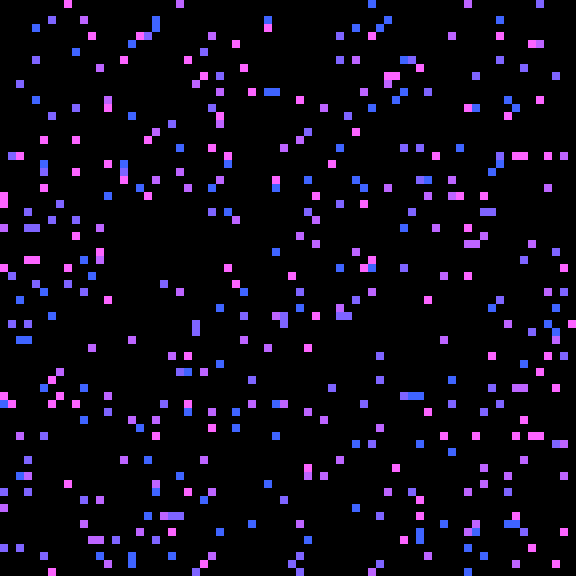
\includegraphics[width=.8\linewidth]{resultados/data/dataset_one/2-0.png} 
    \caption{Primeiro banco de dados. Estado inicial.} 
    \vspace{4ex}
  \end{minipage}%%
  \begin{minipage}[b]{0.5\linewidth}
    \centering
    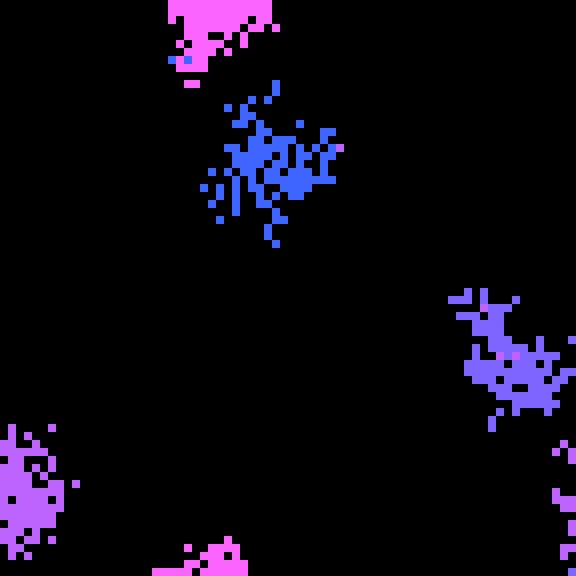
\includegraphics[width=.8\linewidth]{resultados/data/dataset_one/2-1.png} 
    \caption{Primeiro banco de dados. 250.000 passos.} 
    \vspace{4ex}
  \end{minipage} 
  \begin{minipage}[b]{0.5\linewidth}
    \centering
    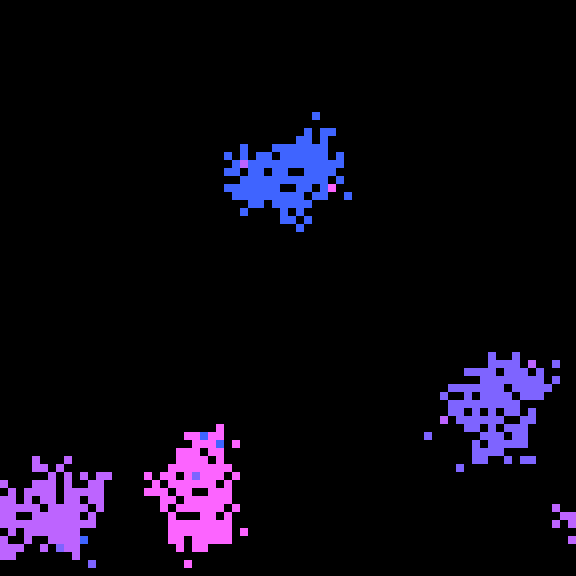
\includegraphics[width=.8\linewidth]{resultados/data/dataset_one/2-2.png} 
    \caption{Primeiro banco de dados. 500.000 passos.} 
    \vspace{4ex}
  \end{minipage}%% 
  \begin{minipage}[b]{0.5\linewidth}
    \centering
    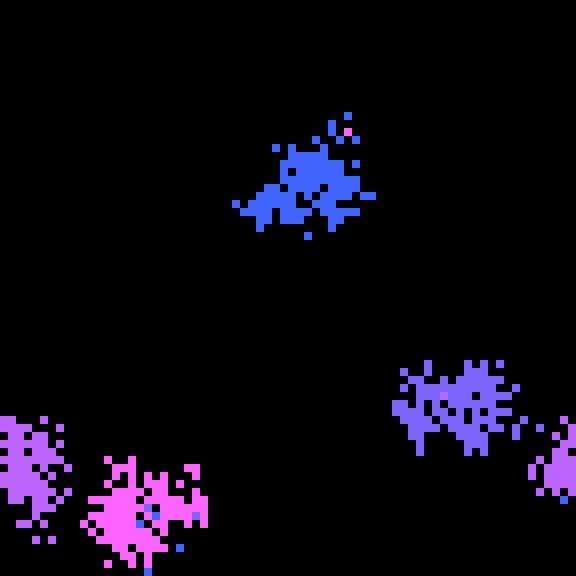
\includegraphics[width=.8\linewidth]{resultados/data/dataset_one/2-3.png} 
    \caption{Primeiro banco de dados. 750.000 passos.} 
    \vspace{4ex}
  \end{minipage}
\end{figure}

O primeiro \textit{dataset} (figura~\ref{fig:dataset_one}) foi executado com as constantes $alpha = 6.5$, $k_1 = 0.75$, $k_2=2.5$ e $R=2$. Mesmo sendo o dataset mais básico, alguns elementos de outros conjuntos ficaram dentro dos conjuntos errados.


\begin{figure}[H] 
  \begin{minipage}[b]{0.5\linewidth}
    \label{fig:dataset_two}
    \centering
    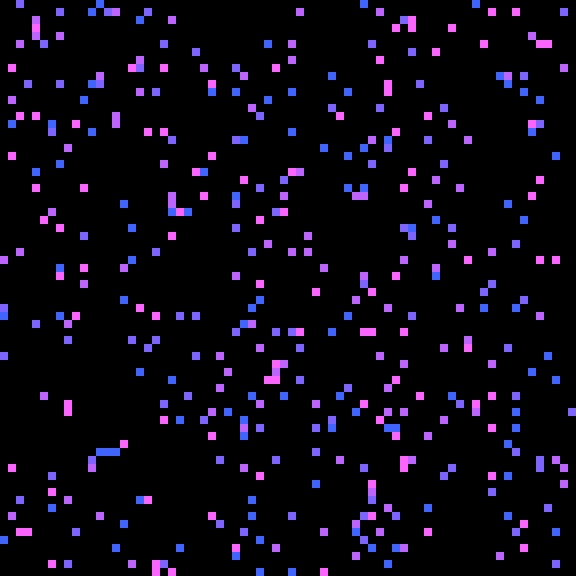
\includegraphics[width=.8\linewidth]{resultados/data/dataset_two/2-0.png} 
    \caption{Segundo banco de dados. Estado inicial.} 
    \vspace{4ex}
  \end{minipage}%%
  \begin{minipage}[b]{0.5\linewidth}
    \centering
    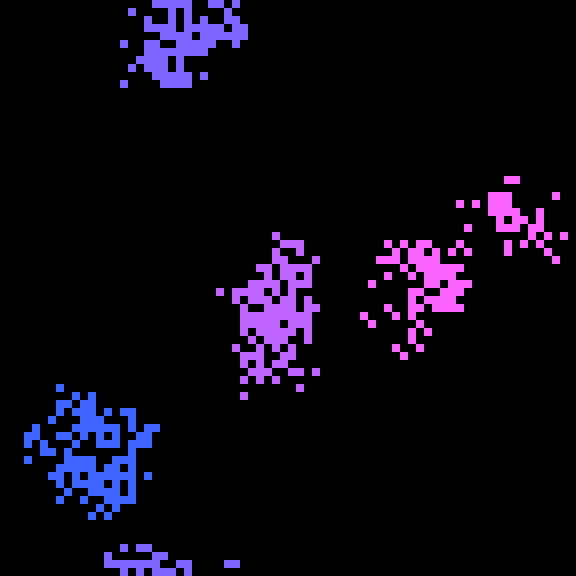
\includegraphics[width=.8\linewidth]{resultados/data/dataset_two/2-1.png} 
    \caption{Segundo banco de dados. 250.000 passos.} 
    \vspace{4ex}
  \end{minipage} 
  \begin{minipage}[b]{0.5\linewidth}
    \centering
    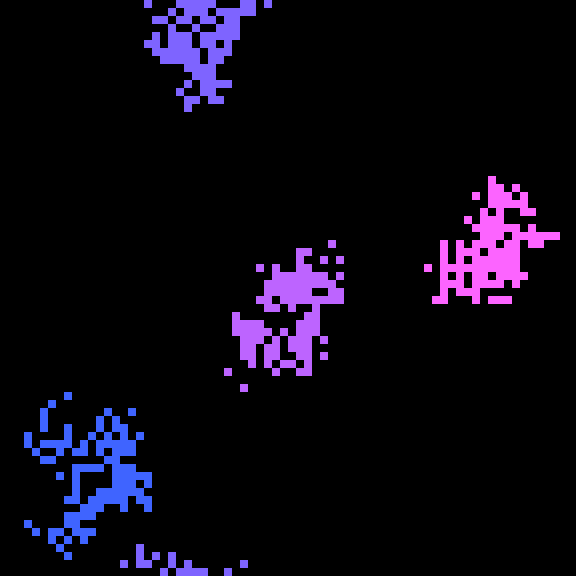
\includegraphics[width=.8\linewidth]{resultados/data/dataset_two/2-2.png} 
    \caption{Segundo banco de dados. 500.000 passos.} 
    \vspace{4ex}
  \end{minipage}%% 
  \begin{minipage}[b]{0.5\linewidth}
    \centering
    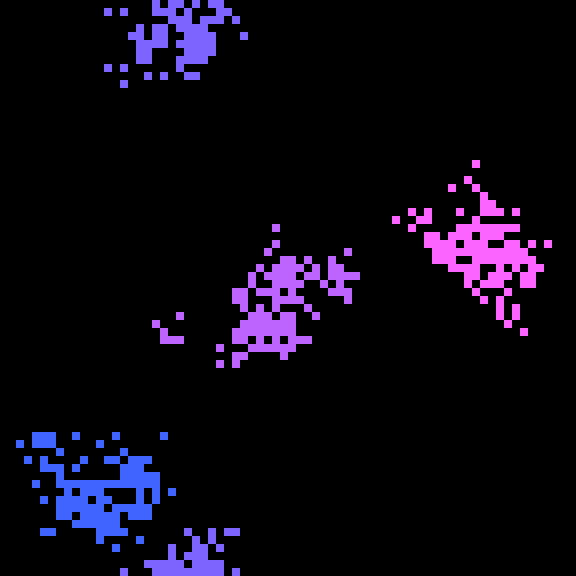
\includegraphics[width=.8\linewidth]{resultados/data/dataset_two/2-3.png} 
    \caption{Segundo banco de dados. 750.000 passos.} 
    \vspace{4ex}
  \end{minipage}
\end{figure}

No segundo \textit{dataset} (Figura~\ref{fig:dataset_two}), o resultado foi ótimo. Nenhum elemento estava dentro de um grupo errado.
As constantes utilizadas foram $alpha=8$, $k_1 = 1$, $k_2 = 1$ e $R=2$.


\begin{figure}[H] 
  \begin{minipage}[b]{0.5\linewidth}
    \label{fig:dataset_three}
    \centering
    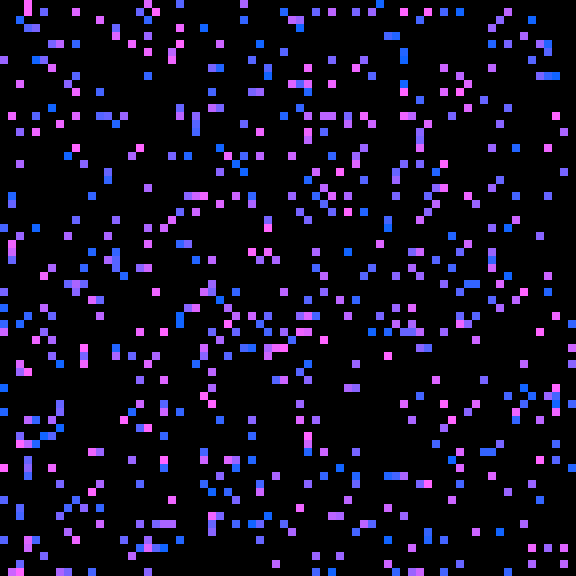
\includegraphics[width=.8\linewidth]{resultados/data/dataset_three/2-0.png} 
    \caption{Terceiro banco de dados. Estado inicial.} 
    \vspace{4ex}
  \end{minipage}%%
  \begin{minipage}[b]{0.5\linewidth}
    \centering
    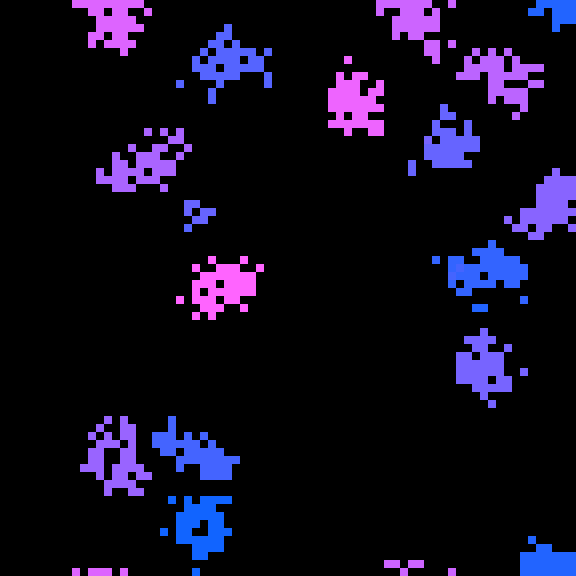
\includegraphics[width=.8\linewidth]{resultados/data/dataset_three/2-1.png} 
    \caption{Terceiro banco de dados. 250.000 passos.} 
    \vspace{4ex}
  \end{minipage} 
  \begin{minipage}[b]{0.5\linewidth}
    \centering
    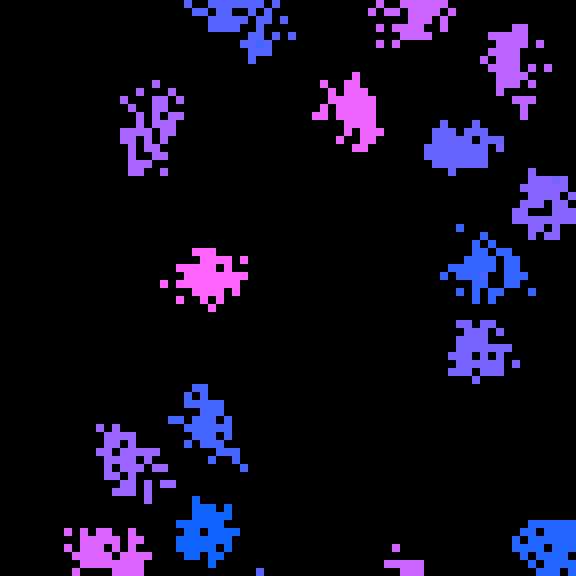
\includegraphics[width=.8\linewidth]{resultados/data/dataset_three/2-2.png} 
    \caption{Terceiro banco de dados. 500.000 passos.} 
    \vspace{4ex}
  \end{minipage}%% 
  \begin{minipage}[b]{0.5\linewidth}
    \centering
    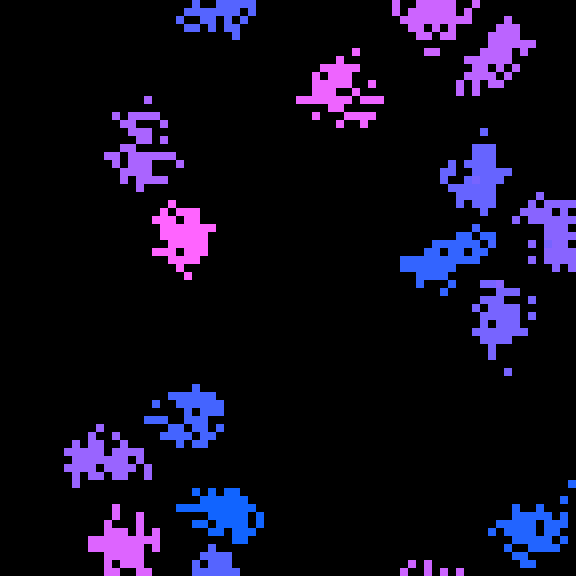
\includegraphics[width=.8\linewidth]{resultados/data/dataset_three/2-3.png} 
    \caption{Terceiro banco de dados. 750.000 passos.} 
    \vspace{4ex}
  \end{minipage}
\end{figure}

No terceiro \textit{dataset} (Figura~\ref{fig:dataset_three}), o resultado foi ótimo. Nenhum elemento estava dentro de um grupo errado. Ressalta-se que este teste era o mais complexo, com 600 elementos e 15 grupos.
As constantes utilizadas foram $alpha=1.2$, $k_1 = 0.3$, $k_2 = 0.6$ e $R=2$.

Não houve, dentre os 3 datasets testados, diferença significativa de desempenho. A média de tempo de execução para 750.000 passos usando $R=2$ é 1min 24.304seg, variando em média 5.326seg de suas extremidades, provavelmente ocorridas pela concorrência de recursos do sistema operacional, como a escrita de arquivos das imagens e gerenciamento das threads.

\section{Conclusão}

Os testes descritos a cima mostram a eficiência de tal sistema para agrupar dados conforme suas categorias. Tal modelagem tem aplicações diretas para utilizar como um sistema de classificação ou análise de dados, como uma base para um sistema de recomendações por exemplo.


\begin{thebibliography}{00}
\bibitem{b1} O. A. Mohamed Jafar, R. Sivakumar, ``Ant-based Clustering Algorithms: A Brief 
Survey'' Phil. International Journal of Computer Theory and Engineering, vol. 2, No. 5, October, 2010.
\bibitem{b2} J. Handl, J. Knowles, M. Dorigo, ``Ant-based clustering: a comparative study of its relative performance with respect to k-means, average link and 1d-som``, Citeseer, 2003, pp.204--213.
\end{thebibliography}

\end{document}
